\documentclass{article}
\usepackage[utf8]{inputenc}
\usepackage{hyperref}
\usepackage{amsmath}
\usepackage{amsfonts}
\usepackage{graphicx}


\title{SPhO Ten Year Series (TYS) with Solutions: 2013 Questions}
\author{
    Solutions available on Victoris\\
    \texttt{victoris.org}
    % new collaborators add your name and contact here!
}

\date{\today}

\begin{document}
\maketitle


\section{2013}

\subsection{Question 1}
1. The first explosion of the atomic bomb was conducted near Alamogoro, New Mexico on July 16, 1945. The Figure below shows a picture of the approximately spherical shockwave $25 \mathrm{~msec}$ with the tick marks indicating $100 \mathrm{~m}$ Using dimensional analysis, find an

\begin{figure}
	\centering
	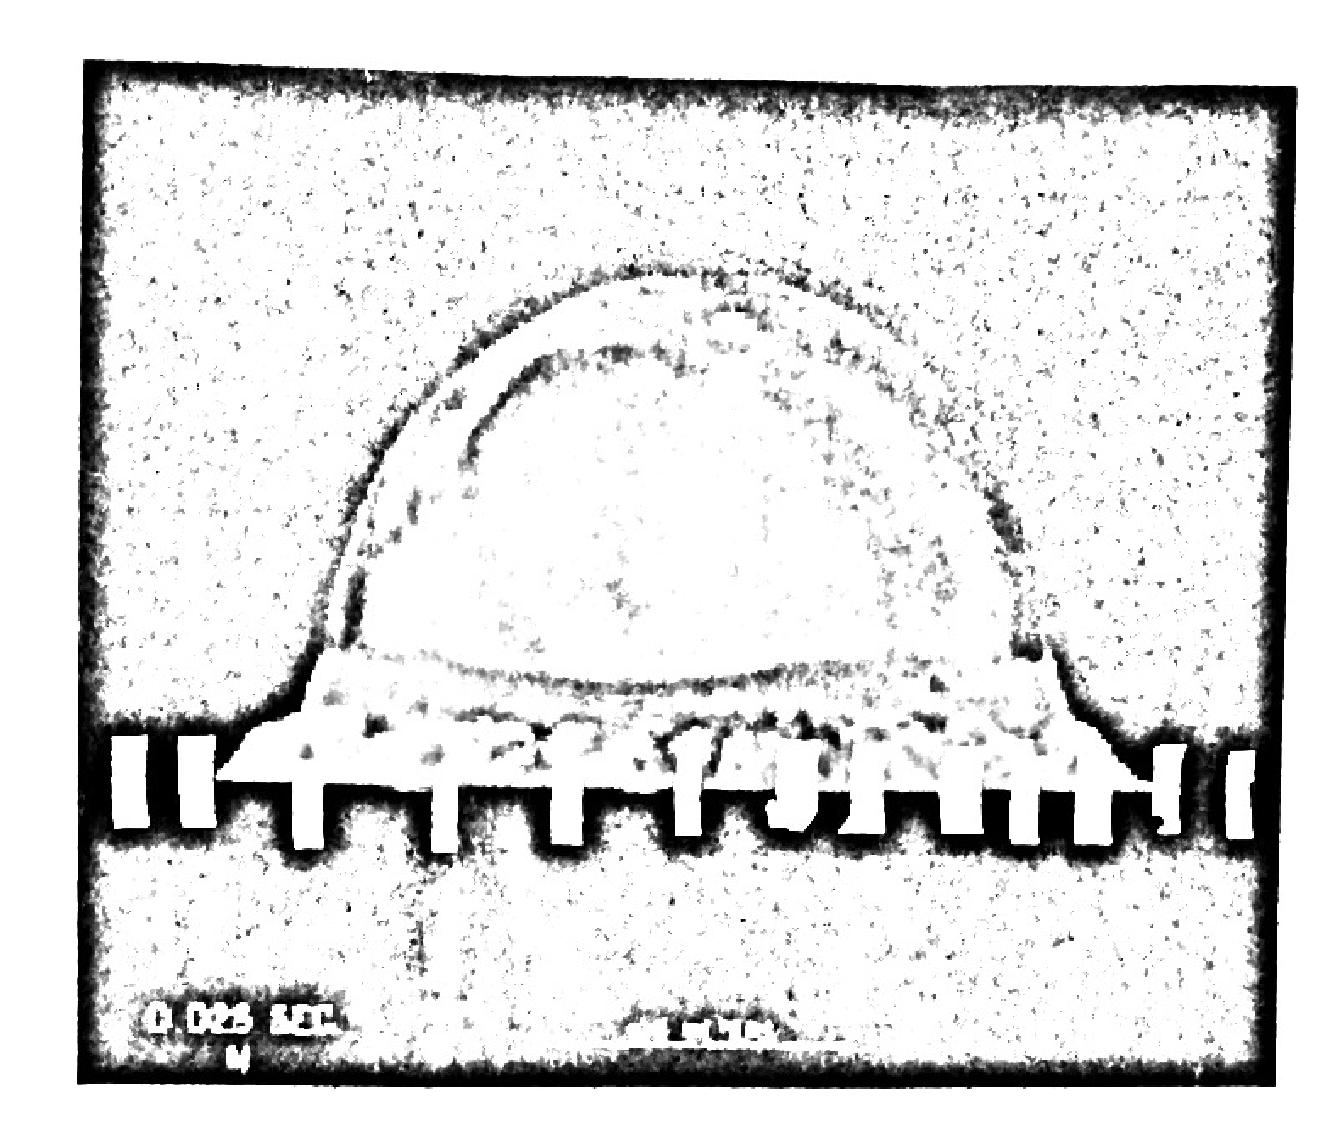
\includegraphics[width=0.5\linewidth]{spho_book_TYS_images/2013q1.png}
	\caption{Camera shot of the bomb after 25 msec.}
\end{figure}

expression for the radius of the shockwave, $R$, as a function of the density $\rho$ of the medium (i.e. the air) through which the shock wave travels, the energy of the explosion, $E$ and the time, $\mathrm{t}$, that elapsed since the explosion.
Assuming that the proportionality constant is unity (i.e. 1), as predicted by Sir Geoffrey Taylor, and assuming that the density of air, $\rho$, is $1.2 \mathrm{~kg} \mathrm{~m}^{-3}$, and that the explosion of $1000 \mathrm{~kg}$ of TNT releases an energy of $4.184 \times 10^{9} \mathrm{~J}$, estimate, from the picture, the approximate energy of this explosion expressed as tons $(1000 \mathrm{~kg})$ of TNT equivalent. [8]

\subsection{Question 2}

2. During a discussion in a physics meeting, Einstein used this problem to illustrate the notion of adiabatic invariant. A pendulum, made up of a ball of mass $M$ suspended from a pivot by a light string of length $L$, is swinging freely in a vertical plane. By what factor does the amplitude of the oscillations change if the string is shortened very slowly by a factor of $2 ?$
$[10]$

\subsection{Question 3}
3. A rocket is projected straight up and explodes into three equally massive fragments just as it reaches the top of its flight. One of the fragments is observed to come straight down to the ground in time $t_{1}$ while the other two land at time $t_{2}$ after the burst. Find the height $h\left(t_{1}, t_{2}\right)$ at which the fragmentation occurred. [10]

\subsection{Question 4}
4. An early but unfortunately incorrect model of the hydrogen atom suggested by J.J. Thomson postulated that the hydrogen atom is a positive cloud of charge $+e$ uniformly distributed throughout a volume of a sphere of radius $R$ with the clectron represented by a equal magnitude but negative point charge $-e$ at the center of the sphere.  \\
(i) Show that the electron is in equilibrium at the center and that if displaced a small distance $r<R$ would experience a restoring force of the form $F=-K r$ where $K$ is a constant. Determine $K$. [3] \\
(ii) Find an expression for the frequency of the simple harmonic oscillations that the electron of mass $m_{e}$ would undergo if displaced a small distance from the center and released. [3] \\
(iii) Calculate a numerical value for $R$ that would result in a frequency of $2.47 \times 10^{15}$ $\mathrm{Hz}$, the frequency of light radiated in the most intense line of the hydrogen spectrum. [3]

\subsection{Question 5}
5. A "perfect" rocket engine combines matter and antimatter in a controlled way to yield photons (high energy gamma rays) all of which are directed out of a spaceship. Suppose we start with a spaceship of initial mass $M_{0}$ at rest, and that at burnout, the remaining spaceship moves at speed $v$ and has mass $m$ equal to the fraction $f$ of the original mass. You may take the speed of light $c=1$ and $\gamma=1 / \sqrt{1-v^{2}}$. \\
(i) What is the total energy of this system initially? Let $E_{\text {rad }}$ stand for the total energy of radiation after the burnout. Find an expression for the total energy of the system after the burnout and set up the conservation of energy equation. [2] \\
(ii) Write down the equation for the conservation of momentum. [2]\\
(iii) Show that $\gamma f+\gamma v f=1$. [2] \\
(iv) Show that $\gamma v=\sqrt{\gamma^{2}-1}$ so that $f^{2}-2 \gamma f+1=0$. [3]
(v) What is the value of $f$ if $\gamma=10 ?$ Is it possible to construct a spaceship whose shell and payload with this $f$? [3] \\
(vi) Using $f$ obtained above for $\gamma=10$, show that the total energy of the emitted radiation is less than the mass of fuel consumed. Explain why. [3]


\subsection{Question 6}
6. On a smooth and insulating large ring of radius $R$, there is a small ring of mass $m$ and carrying charge $q$. The large ring is placed horizontally and in a uniform magnetic field of strength $B_{0}$ and perpendicular to the ring plane. Starting at $t=0$, the magnetic field is changed to $B(t)=B_{0}+\alpha t$. Find the force of the small ring acting on the big ring afterwards and describe the motion of the small ring [10]

\subsection{Question 7}
7. Three polarizing disks whose planes are parallel are centered on a common axis. The direction of the transmission axis in each case is shown in Figure 2 relative to the common vertical direction. A plane-polarized beam of light with $E_{0}$ parallel to the vertical reference direction is incident from the left on the first disk with intensity $I_{0}=10.0$ in some arbitrary units. Calculate the transmitted intensity I when
(i) $\theta_{1}=20.0^{\circ}, \theta_{2}=40.0^{\circ}$, and $\theta_{3}=60.0^{\circ} ;$
(ii) $\theta_{1}=0^{\circ}, \theta_{2}=30.0^{\circ}$, and $\theta_{3}=60.0^{\circ} ;$
(iii) If $\theta_{1}=0^{\circ}$ and $\theta_{3}=60.0^{\circ}$, find the angle $\theta_{2}$ so that maximum intensity passes through the three polarizers.

\begin{figure}
	\centering
	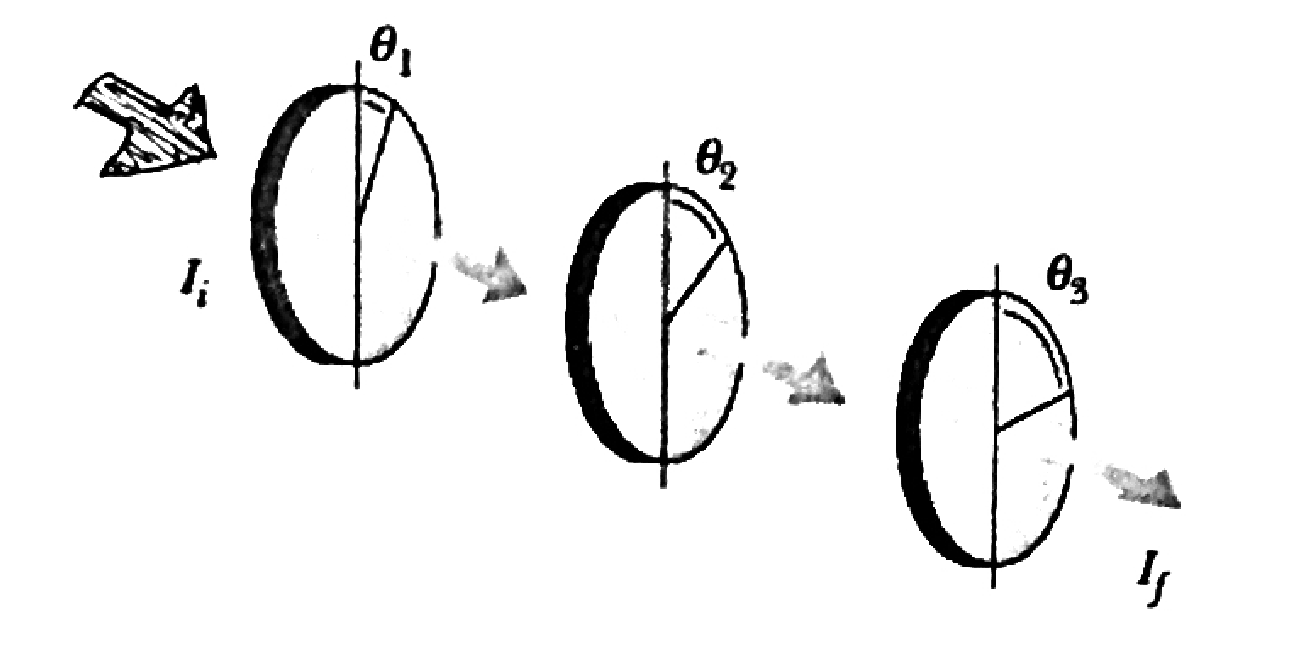
\includegraphics[width=0.5\linewidth]{spho_book_TYS_images/2013q7.png}
	\caption{Three polarizing disks whose planes are parallel are centered on a common axis.}
\end{figure}


\subsection{Question 8}
8. Two parallel rails with negligible resistance are $10.0 \mathrm{~cm}$ apart and are connected by a $5.00 \Omega$ resistor. The circuit also contains two metal rods having resistances of $10.0$ $\Omega$ and $15.0 \Omega$ sliding along the rails (see figure 3). The rods are pulled away from the resistor at constant speeds of $4.00 \mathrm{~ms}^{-1}$ and $2.00 \mathrm{~ms}^{-1}$, respectively. A uniform magnetic field of magnitude $0.0100 \mathrm{~T}$ is applied perpendicular to the plane of the rails. Determine the current in the $5.00 \Omega$ resistor. [8]


\subsection{Question 9}
9. In the figure below, the switch is closed for $t<0$, and steady-state conditions are established. The switch is opened at $t=0$.\\
(i) Find the initial voltage $\mathcal{E}_{t}$ across $L$ just after $t=0$. Which end of the coil is $\mathrm{nt}$ the higher potential: a or b? [3]\\
(ii) Sketch graphs of the currents in $R_{1}$ and in $R_{2}$ as a function of time, treating the steady-state directions as positive. Show the values before and after $t=0$. [5] \\
(iii) How long after $t=0$ would the current across $R_2$ be $2.00 \mathrm{~mA}$? [2]


\begin{figure}
	\centering
	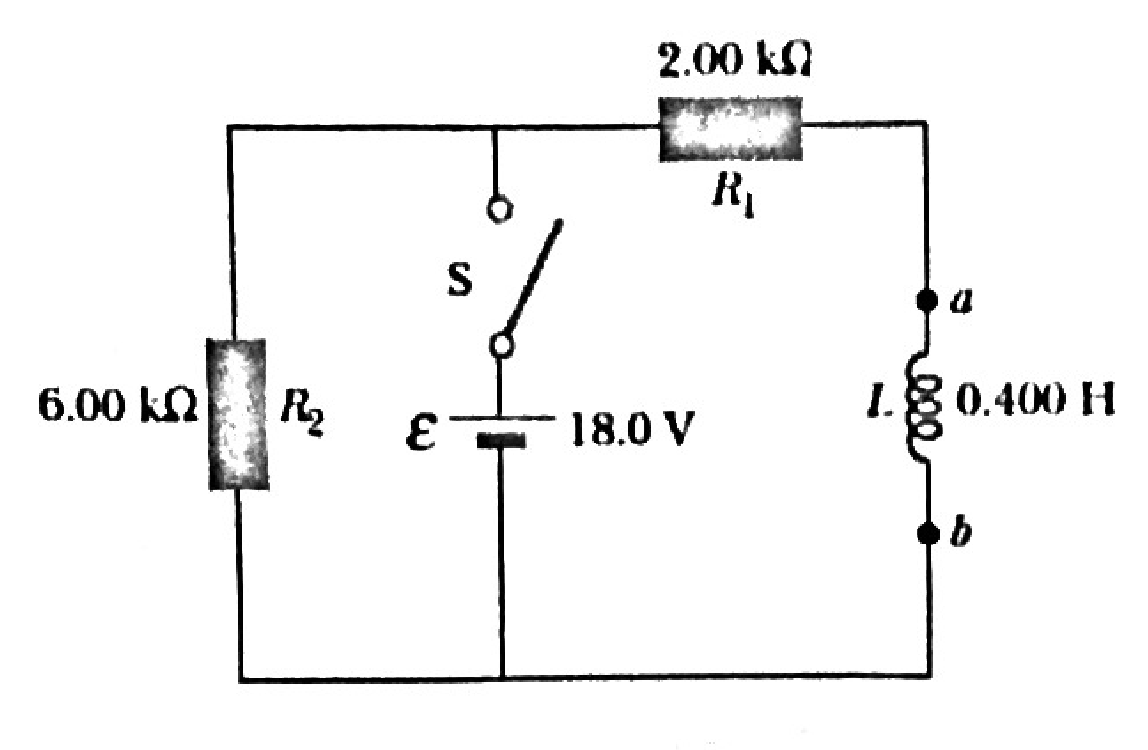
\includegraphics[width=0.5\linewidth]{spho_book_TYS_images/2013q9.png}
	\caption{Circuit}
\end{figure}

\subsection{Question 10}
10. A transparent cylinder of radius $R=2.00$ m has a mirrored surface on its right half, as shown in Figure 5. A light ray traveling in air is incident on the left side of the cylinder. The incident light ray and exiting light ray are parallel and $d=2.00 \mathrm{~m}$. Determine the index of refraction of the material. [10]

\begin{figure}
	\centering
	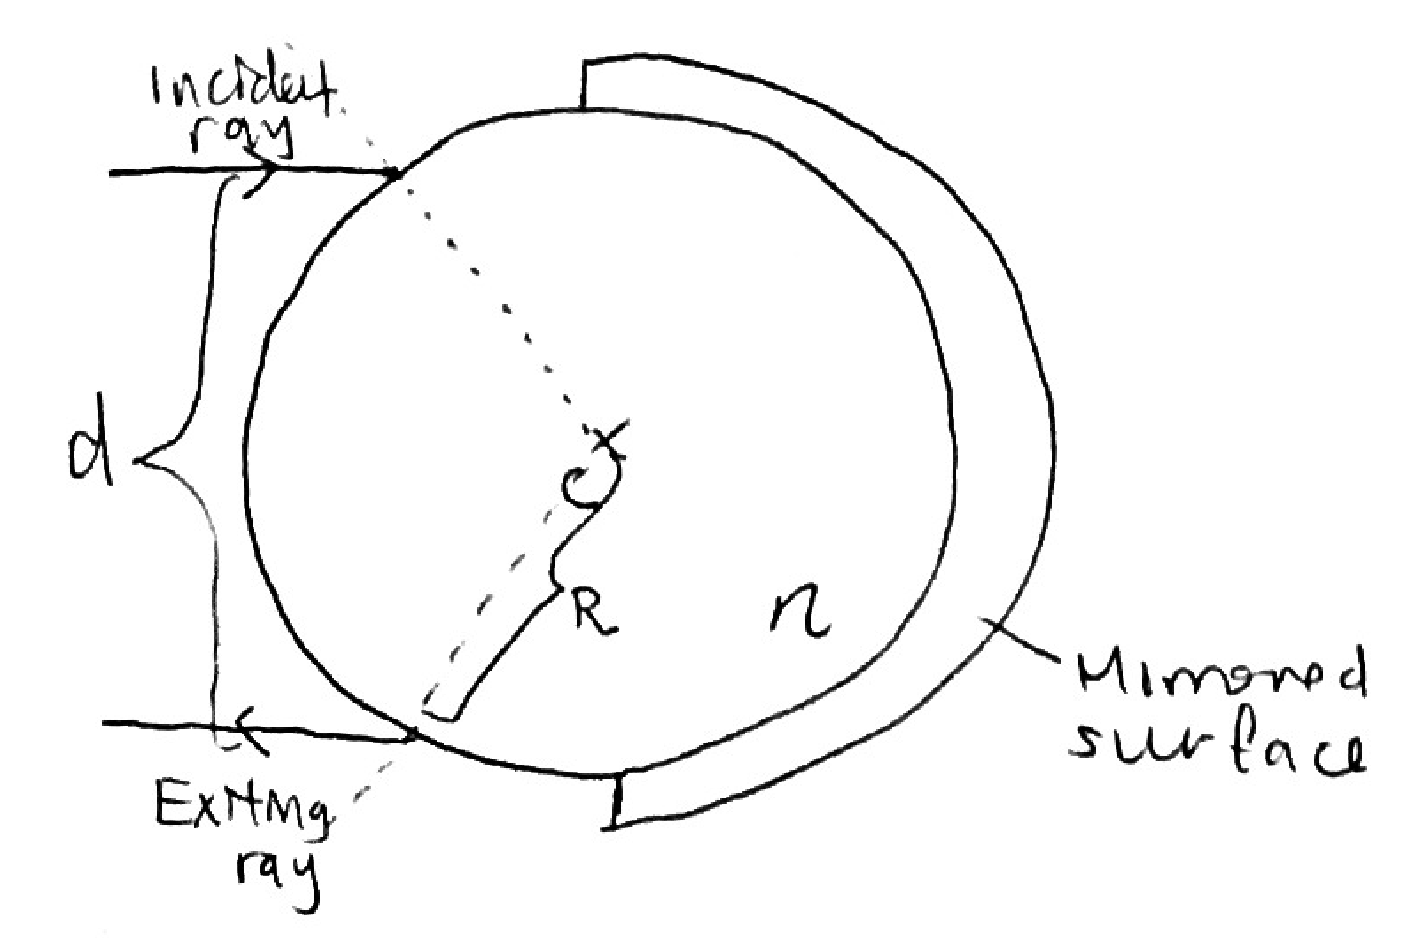
\includegraphics[width=0.5\linewidth]{spho_book_TYS_images/2013q10.png}
	\caption{Transparent cylinder with mirrored surface}
\end{figure}


\end{document}
